\documentclass[
    alternativetitlepage=alternativ,
    cornerlogo=hgi_nds_logo2,
    sectionoverview,
]{rubpresentation}
\setbeamercovered{invisible}

\title[XML/JSON conversions]
{Bridging the Gap: Secure and lossless conversion\\ of XML data structures to the JSON format}
\subtitle{\small Bachelor thesis \hspace{3mm}{\scriptsize $\blacksquare$}\hspace{3mm} March 30, 2017 -- June 29, 2017}

\author[Holthuis]{Jan~Holthuis}

\institute[Advisors]
{%\inst{1}%
Advisors: Dennis Felsch \& Paul Rösler
}
\date{June 06, 2017}
\subject{Computer Science}

\titlegraphic{titlepage.png}
\sponsorlogo[height=7.6mm,interpolate=true]{hgi_nds_logo}

\definecolor{diffstart}{named}{blue}
\definecolor{diffincl}{named}{green}
\definecolor{diffrem}{named}{red}

\usepackage{listings}
  \lstdefinelanguage{diff}{
    basicstyle=\ttfamily\small,
    morecomment=[f][\color{diffstart}]{@@},
    morecomment=[f][\color{diffincl}]{+\ },
    morecomment=[f][\color{diffrem}]{-\ },
  }

\begin{document}

\frame[plain]{\titlepage}

%\begin{frame}{The \texttt{\textbackslash note}-Macro}
%\begin{itemize}[<+->]
%\item normal text for the presentation.
%\note<1-2>[item]{Say something to the audience!}
%\item and text for the presentation.
%\item foo
%\end{itemize}
%\note<2>{Another note for you!}
%\end{frame}

%\note[enumerate]{\item foo \item bar \item baz \item foobar}


\section{Quick Recap}

\begin{frame}
    \frametitle{Last time we learned that\dots{}}
    \framesubtitle{}
    \begin{itemize}
        \item{} Based on my current conversion critera, \emph{no existing solution} allows lossless XML$\rightarrow$JSON$\rightarrow$XML roundtrips\dots{}
        \item{} \dots{}but I found a promising candidate named \textbf{JsonML}
        \begin{itemize}
            \item{} Handles most stuff correctly
            \item{} Resulting JSON is not very friendly because it uses Arrays almost for everything
            \item{} Multiple implementations exist
        \end{itemize}
    \end{itemize}
\end{frame}


\section{Progress report}

\begin{frame}[fragile]
    \frametitle{Progress made in the last two weeks}
    \framesubtitle{Complex tests}
    \begin{itemize}
        \item{} Most of my existing tests concentrate on small, isolated conversion problems
        \item{} Now I added some \enquote{real-world} examples
        \begin{itemize}
            \item{} The official sample documents for RSS version 0.91, 0.92 and 2.0
            \item{} The XML 1.0 specification as XML and XHTML
            \item{} Two SVG images from the W3 SVG Web toolkit (one of them has embedded JavaScript)
            \item{} The resulting XML of an API call to the MusicBrainz.org Web Service v2
            \item{} The ODF v1.0 (Second Edition) specification in Flat OpenDocument Text format (*.fodt)
        \end{itemize}
    \end{itemize}
\end{frame}

\begin{frame}[fragile]
    \frametitle{Progress made in the last two weeks}
    \framesubtitle{Character support tests}
    \begin{itemize}
        \item{} Added a bunch of character support tests
    \end{itemize}
    \begin{lstlisting}[basicstyle=\fontsize{7}{11}\ttfamily,numbers=none]
\$ ls -l code/test-documents/charsupport/
total 1048
-rw-r--r-- 1 jan jan    258 May 25 16:03 chars-u000009-u00000D.xml.testcase
-rw-r--r-- 1 jan jan   1374 May 25 00:19 chars-u000020-u00007E.xml.testcase
-rw-r--r-- 1 jan jan    304 May 25 00:19 chars-u00007F-u000084.xml.testcase
-rw-r--r-- 1 jan jan    609 May 25 00:19 chars-u000080-u00009F.xml.testcase
-rw-r--r-- 1 jan jan    565 May 25 00:19 chars-u000086-u00009F.xml.testcase
-rw-r--r-- 1 jan jan 982708 May 25 00:19 chars-u0000A0-u00D7FF.xml.testcase
-rw-r--r-- 1 jan jan    802 May 25 00:19 chars-u00FDD0-u00FDEF.xml.testcase
-rw-r--r-- 1 jan jan    267 May 25 00:19 chars-u01FFFE-u01FFFF.xml.testcase
-rw-r--r-- 1 jan jan    267 May 25 00:19 chars-u02FFFE-u02FFFF.xml.testcase
-rw-r--r-- 1 jan jan    267 May 25 00:19 chars-u03FFFE-u03FFFF.xml.testcase
-rw-r--r-- 1 jan jan    267 May 25 00:19 chars-u04FFFE-u04FFFF.xml.testcase
-rw-r--r-- 1 jan jan    267 May 25 00:19 chars-u05FFFE-u05FFFF.xml.testcase
[...]
-rw-r--r-- 1 jan jan    267 May 25 00:19 chars-u0FFFFE-u0FFFFF.xml.testcase
-rw-r--r-- 1 jan jan    271 May 25 00:19 chars-u10FFFE-u10FFFF.xml.testcase
    \end{lstlisting}
\end{frame}

\section{The curious case of the \texttt{>} character}

\begin{frame}
    \frametitle{The curious case of the \texttt{>} character}
    \framesubtitle{Escaping}
    \begin{itemize}
        \item{} Want a \texttt{<} char in a text node (not \texttt{CDATA})? Escape it! $\Rightarrow$ \texttt{\&lt;}
        \item{} What about \texttt{>}?
        \begin{itemize}
            \item{} Escaping it to \texttt{\&gt;} is not necessary\dots{}
            \item{} \dots{} \textbf{except} \enquote{when it appears in the string \enquote{\texttt{]]>}} in content, when that string is not marking the end of a CDATA section.} (XML 1.0, Section 2.4).
        \end{itemize}
    \end{itemize}
\end{frame}

\begin{frame}[fragile]
    \frametitle{The curious case of the \texttt{>} character}
    \framesubtitle{Why does this matter?}
    \begin{itemize}
        \item{} Two JavaScript-based converters failed this test:
        \begin{itemize}
            \item{} JsonML
            \item{} JXON
        \end{itemize}
        \item{} Both are using \texttt{DOMParser} for XML, which part of the Browser-only Web API
        \begin{itemize}
            \item{} JXON is using the \texttt{xmldom} Node.js implementation
            \item{} JsonML is browser-only, so I added \texttt{xmldom} support using monkey patch for easier testing on the CLI
        \end{itemize}
    \end{itemize}
\end{frame}

\begin{frame}[fragile]
    \frametitle{The curious case of the \texttt{>} character}
    \framesubtitle{JsonML-\texttt{xmldom} glue}
    \begin{lstlisting}[basicstyle=\fontsize{7}{11}\ttfamily,numbers=none]
    /* Create fake browser context by using methods from xmldom module */
    const ctx = {
        "DOMParser": xmldom.DOMParser,
        "document": (new xmldom.DOMParser()).parseFromString("<x/>", "text/xml"),
        "window": {
            "DOMParser": xmldom.DOMParser,
            "XMLSerializer": xmldom.XMLSerializer,
        },
    };
    /* Run code in fake browser context */
    let filename = require.resolve("jsonml-tools/jsonml-xml.js")
    let code = fs.readFileSync(filename, "utf-8");
    vm.runInNewContext(code, ctx);
    \end{lstlisting}
\end{frame}

\begin{frame}
    \frametitle{The curious case of the \texttt{>} character}
    \framesubtitle{Investigating the problem}
    \begin{itemize}
        \item{} Both \texttt{xmldom}-using converters fail. Coincidence?
        \item{} Found out that there was a regression in \texttt{xmldom}\dots{}
        \item{} \dots{} so \texttt{xmldom} was the cause of the problem.
        \item{} A commit from 2012 (!) broke this behaviour
        \item{} There was a unittest, but the commit broke that too
        \item{} $\Rightarrow$ I wrote a patch to make \texttt{xmldom} great again
    \end{itemize}
\end{frame}

\begin{frame}[fragile]
    \frametitle{The curious case of the \texttt{>} character}
    \framesubtitle{Patching xmldom}
    \begin{lstlisting}[language=diff,basicstyle=\fontsize{7}{11}\ttfamily,numbers=none]
diff --git a/dom.js b/dom.js
@@ -1053,7 +1053,7 @@ function serializeToString(node,buf,isHTML,nodeFilter,visibleNamespaces){
   case TEXT_NODE:
-     return buf.push(node.data.replace(/[<\&]/g,_xmlEncoder));
+     return buf.push(node.data.replace(/[<\&]/g,_xmlEncoder).replace(/\]\]>/g,']]'+_xmlEncoder('>')));
diff --git a/test/dom/serializer.js b/test/dom/serializer.js
@@ -5,7 +5,7 @@ wows.describe('XML Serializer').addBatch({
   'text node containing "]]>"': function() {
     var doc = new DOMParser().parseFromString('<test/>', 'text/xml');
     doc.documentElement.appendChild(doc.createTextNode('hello ]]> there'));
-    console.assert(doc.documentElement.firstChild.toString() == 'hello ]]> there',doc.documentElement.firstChild.toString());
+    console.assert(doc.documentElement.firstChild.toString() == 'hello ]]\&gt; there',doc.documentElement.firstChild.toString());
   },
    \end{lstlisting}
\end{frame}

\section{Next steps}

\begin{frame}
    \frametitle{Next Steps}
    \begin{itemize}
        \item{} Continue writing
        \item{} ???
        \item{} Profit!
    \end{itemize}
\end{frame}

\section{Commercial break}

\begin{frame}
    \frametitle{Nice formatting style for \LaTeX's \texttt{minted}}
    \framesubtitle{(Shameless Self-Advertising)}
    \begin{itemize}
        \item{} You use the RUB thesis \LaTeX{} template?
        \item{} You need nice code listings (using the \texttt{minted} package) that \textbf{use the RUB corporate design colors?}
        \item{} Check out the \texttt{rub} style from \texttt{github.com/Holzhaus/pygments-style-rub}!
    \end{itemize}
    \begin{center}
        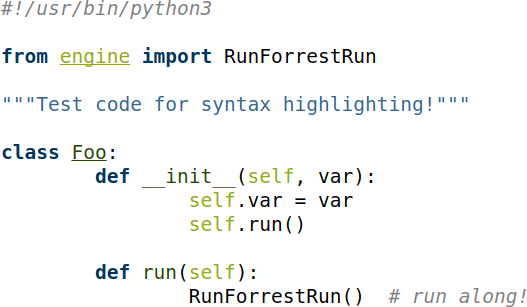
\includegraphics[height=4.2cm]{rubmintedstyle}
    \end{center}
\end{frame}

%%% Finally the last slide

\begin{frame}[plain]
\frametitle{Thanks!}
 \begin{center}
 {\bfseries\fontsize{30pt}{1.2em}\selectfont Questions?}
 \end{center}
  \begin{columns}
    \begin{column}{0.5\textwidth}
      \begin{center}
        %\font\endfont = cmss10 at 25.40mm
        %\color{Brown}
        %\endfont
        %\baselineskip 20.0mm
        Reach out via email:
        \begin{itemize}
        \item \textbf{Jan Holthuis}\\
              jan.holthuis@rub.de
        \end{itemize}
      \end{center}
    \end{column}
    \begin{column}{0.5\textwidth}
      \begin{center}
        \pgfimage[width=\textwidth]{questions.jpg}
      \end{center}
    \end{column}
  \end{columns}
\end{frame}

\end{document}
